\documentclass[11pt,mathserif]{beamer}

%% paketeak
\usepackage{amsmath,amssymb,amsfonts,amsthm}
\usepackage{svg}
\usepackage{graphicx}
\usepackage{bbding}
\usepackage{fontawesome}
\usepackage[utf8]{inputenc}
\usepackage[french]{babel}
\usepackage{fancyvrb}
\usepackage{relsize}
\usepackage{color}
\usepackage{listings}
\usepackage{caption}
\usepackage{bbold}
\usepackage{tikz}
\usepackage[absolute,overlay]{textpos}
\usepackage{ifthen}
% kolore batzuk definitu
\definecolor{dkgreen}{rgb}{0,0.6,0}
\definecolor{gray}{rgb}{0.5,0.5,0.5}
\definecolor{mauve}{rgb}{0.58,0,0.82}
\definecolor{bleuSympa}{rgb}{0.,0.19,0.607}
\definecolor{arrosa}{rgb}{0.7,0.15,0.15}

% bidexka erabilgarriak fontawesome erabiltzen
\renewcommand{\thefootnote}{$\dagger$}
\newcommand{\scout}{\faAngellist}
\newcommand{\gezi}{\faLongArrowRight}
\newcommand{\galde}{\faQuestion}
\newcommand{\bof}{\faMehRollingEyes[regular]}
\newcommand{\hand}{\faHandORight}
\newcommand{\argi}{\faLightbulbO}
\newcommand{\Pdf}{\faFilePdfO}
\newcommand{\liburu}{\faBook}
\newcommand{\kontuz}{\faExclamationTriangle}
\newcommand{\pozik}{\faSmileO}
\newcommand{\triste}{\faFrownO}
\newcommand{\egia}{\faCheckCircle}
\newcommand{\adibi}{\faCommentO}
\newcommand{\harritu}{\faExclamation}
\newcommand{\geldi}{\faHandPaperO}
\captionsetup[figure]{labelformat=empty}
\newcommand{\geziBikoitz}{\faArrowsH}

% c/fortran aukeratzeko
\newif\ifC
\ifthenelse{\equal{\detokenize{c}}{\jobname}}{
  \Ctrue
}{
  \Cfalse
}
\ifC
  \newcommand{\mylang}{c}
  \newcommand{\othlang}{fortran}
  \newcommand{\extlang}{c}
  \newcommand{\extcu}{cu}
  \newcommand{\lstemphcu}{__global__, __shared__, __device__, __host__, __syncthreads, threadIdx, blockIdx, blockDim, gridDim}
  \newcommand{\spt}{.}
\else
  \newcommand{\mylang}{fortran}
  \newcommand{\othlang}{c}
  \newcommand{\extlang}{f90}
  \newcommand{\extcu}{cuf}
  \newcommand{\lstemphccu}{global, shared, device, host, syncthreads, attributes, threadIdx, blockIdx, blockDim, gridDim}
  \newcommand{\spt}{\%}
\fi
\newcommand{\includeSrc}[1]{\lstinputlisting[language=\mylang]{#1.\extlang}}
\newcommand{\includeSrcCu}[1]{\lstinputlisting{#1.\extcu}}

% listings CUDA lengoaia kudeatzeko
\lstset{ %
  numbers=none,
  numbersep=1pt,
  numberstyle=\relsize{-5}\ttfamily,
  language=\mylang,                % the language of the code
  framerule=1pt,
  basicstyle=\relsize{-3}\ttfamily,           % the size of the fonts that are used for the code
                                  % will be numbered
  %numbersep=5pt,                  % how far the line-numbers are from the code
  backgroundcolor=\color{black!20},      % choose the background color. You must add \usepackage{color}
  showspaces=false,               % show spaces adding particular underscores
  showstringspaces=false,         % underline spaces within strings
  showtabs=false,                 % show tabs within strings adding particular underscores
  %frame=single,                   % adds a frame around the code
  rulecolor=\color{black},        % if not set, the frame-color may be changed on line-breaks within not-black text (e.g. commens (green here))
  %tabsize=2,                      % sets default tabsize to 2 spaces
  breaklines=true,                % sets automatic line breaking
  breakatwhitespace=false,        % sets if automatic breaks should only happen at whitespace
  lineskip=-1pt,
  emph={\lstemphcu},
  keywordstyle=\color{bleuSympa}\textbf,          % keyword style
  commentstyle=\color{bleuSympa},       % comment style
  stringstyle=\color{mauve},
  emphstyle=\color{arrosa},
  moredelim=[s][\color{arrosa}\ttfamily]{<<<}{>>>},
  morecomment=[s][\color{mauve}]{cudaMemcpyHostToDevice}{\ },
  morecomment=[s][\color{mauve}]{cudaMemcpyDeviceToHost}{\ }
}

%% ====== nire beamer estiloa
\defbeamertemplate{itemize item}{boldarrow}{\raisebox{0.3ex}{\resizebox{1.2ex}{1ex}{\ArrowBoldRightShort}}}
\mode<presentation> {
\usetheme{default}    % urri
\useinnertheme[shadow]{rounded}  % zenbakiak biribiltzeko
}
\usefonttheme{structurebold}

\begin{document}
\begin{frame}{Présentation du materiel}
  \begin{itemize}[<+->]
    \item GPU dispos : k40m
    \item hôte : machine accessible en ssh au travers de l'ordonnanceur SLURM
\pause
 \begin{center}
   \colorbox{white}{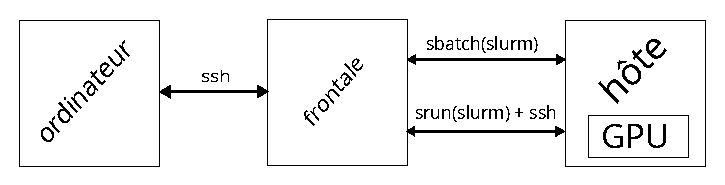
\includegraphics[width=0.7\linewidth]{fig/schema_slurm.eps}}
 \end{center}
    \item 2 modes pour utiliser les GPUs
      \begin{itemize}
        \item interactif : {\tt salloc -N 1 -q cytech --time 0:5:0 } puis {\tt ssh nom\_hôte}
        \item par lot : {\tt sbatch mon\_fichier.sl }
      \end{itemize}
  \end{itemize}
\end{frame}
\begin{frame}{Charger l'environnement}
\begin{itemize}
  \item copier le fichier de config dans votre répertoire : \lstinline$cp ~fuentes/load\_env* .$ 
  \item charger le fichier de config : 
  \item vérifier le chemin vers le compilateur \lstinline$which nvcc$
\lstinputlisting{code/chemin_nvcc}
  \item lancer nvaccelinfo (ou nvidia-smi)
\lstinputlisting[numbers=none,language=bash,basicstyle=\relsize{-4}\ttfamily]{code/nvaccel}
  \item trouver les infos suivantes
  \begin{itemize}
    \item nombre d'accelerateurs
    \item nombre de SM
    \item nombre max de «threads» par bloc
  \end{itemize}
\end{itemize}
\end{frame}
\begin{frame}{Premier programme}
\begin{itemize}
  \item écrire un programme "bonjour, monde"
\lstinputlisting{code/bonjour.c}
  \item le compiler et l'executer \lstinline$nvcc -cuda -gpu=cc75 bonjour.c && ./a.out $
\lstinputlisting[numbers=none,language=bash,basicstyle=\relsize{-4}\ttfamily]{code/bonjourOut}
\end{itemize}
\end{frame}
% programme increment
\begin{frame}{noyau homothétie}
\begin{itemize}[<+->]
  \item Soit le code CPU d'homothétie suivante
\lstinputlisting{code/homothetie.c}
  \item implanter une version GPU
  \item implanter une version avec saut `scaleFlipAndHalf` comme dans le cours
  \item utiliser les evenements pour chronometrer les temps d'execution des noyaux
\end{itemize}
\end{frame}

\end{document}
